
%-----------------------------------------------------------------------------
% PACKAGES AND OTHER DOCUMENT CONFIGURATIONS
%-----------------------------------------------------------------------------

\documentclass[11pt]{exam}

\usepackage[margin=1in]{geometry}
\usepackage{amsmath, amsfonts}
\usepackage{enumerate}
\usepackage{graphicx}
\usepackage{titling}
\usepackage{url}
\usepackage{xfrac}
\usepackage{geometry}
\usepackage{graphicx}
\usepackage{natbib}
\usepackage{amsmath}
\usepackage{amssymb}
\usepackage{amsthm}
\usepackage{paralist}
\usepackage{epstopdf}
\usepackage{tabularx}
\usepackage{longtable}
\usepackage{multirow}
\usepackage{multicol}
\usepackage[colorlinks=true,urlcolor=blue]{hyperref}
\usepackage{algorithm}
\usepackage{algorithmicx}
\usepackage[noend]{algpseudocode}
\usepackage{float}
\usepackage{paralist}
\usepackage[svgname]{xcolor}
\usepackage{enumerate}
\usepackage{array}
\usepackage{times}
\usepackage{url}
\usepackage{comment}
\usepackage{environ}
\usepackage{times}
\usepackage{textcomp}
\usepackage{caption}
\usepackage[colorlinks=true,urlcolor=blue]{hyperref}
\usepackage{parskip} % For NIPS style paragraphs.
\usepackage[compact]{titlesec} % Less whitespace around titles
\usepackage[inline]{enumitem} % For inline enumerate* and itemize*
\usepackage{datetime}
\usepackage{comment}
% \usepackage{minted}
\usepackage{lastpage}
\usepackage{color}
\usepackage{xcolor}
\usepackage[final]{listings}
\usepackage{tikz}
\usetikzlibrary{shapes,decorations}
\usepackage{framed}
\usepackage{booktabs}
\usepackage{cprotect}
\usepackage{fancyvrb}
\usepackage{xcolor}
\usepackage{verbatimbox}
\usepackage[final]{listings}
\usepackage{bm}
\usepackage{hyperref}
\usepackage{subcaption}
\usepackage{mathtools} % For drcases
\usepackage{cancel}
\usepackage[many]{tcolorbox}
\usepackage{soul}

\usepackage{cancel}

%%%%%%%%%%%%%%%%%%%%%%%%%%%%%%%%%%%%%%%%%%%
% Better numbering                        %
%%%%%%%%%%%%%%%%%%%%%%%%%%%%%%%%%%%%%%%%%%%

\numberwithin{equation}{section} % Number equations within sections (i.e. 1.1, 1.2, 2.1, 2.2 instead of 1, 2, 3, 4)
\numberwithin{figure}{section} % Number figures within sections (i.e. 1.1, 1.2, 2.1, 2.2 instead of 1, 2, 3, 4)
\numberwithin{table}{section} % Number tables within sections (i.e. 1.1, 1.2, 2.1, 2.2 instead of 1, 2, 3, 4)

%%%%%%%%%%%%%%%%%%%%%%%%%%%%%%%%%%%%%%%%%%
% Custom commands                        %
%%%%%%%%%%%%%%%%%%%%%%%%%%%%%%%%%%%%%%%%%%

\def\x{\mathbf x}
\def\y{\mathbf y}
\def\w{\mathbf w}
\def\v{\mathbf v}
\def\E{\mathbb E}
\def\V{\mathbb V}
\newcommand{\blackcircle}{\tikz\draw[black,fill=black] (0,0) circle (1ex);}
\renewcommand{\circle}{\tikz\draw[black] (0,0) circle (1ex);}
\newcommand{\vc}[1]{\boldsymbol{#1}}
\newcommand{\adj}[1]{\frac{d \ell}{d #1}}
\newcommand{\chain}[2]{\adj{#2} = \adj{#1}\frac{d #1}{d #2}}
\newcommand{\ntset}{test}

% mathcal
\newcommand{\Ac}{\mathcal{A}}
\newcommand{\Bc}{\mathcal{B}}
\newcommand{\Cc}{\mathcal{C}}
\newcommand{\Dc}{\mathcal{D}}
\newcommand{\Ec}{\mathcal{E}}
\newcommand{\Fc}{\mathcal{F}}
\newcommand{\Gc}{\mathcal{G}}
\newcommand{\Hc}{\mathcal{H}}
\newcommand{\Ic}{\mathcal{I}}
\newcommand{\Jc}{\mathcal{J}}
\newcommand{\Kc}{\mathcal{K}}
\newcommand{\Lc}{\mathcal{L}}
\newcommand{\Mc}{\mathcal{M}}
\newcommand{\Nc}{\mathcal{N}}
\newcommand{\Oc}{\mathcal{O}}
\newcommand{\Pc}{\mathcal{P}}
\newcommand{\Qc}{\mathcal{Q}}
\newcommand{\Rc}{\mathcal{R}}
\newcommand{\Sc}{\mathcal{S}}
\newcommand{\Tc}{\mathcal{T}}
\newcommand{\Uc}{\mathcal{U}}
\newcommand{\Vc}{\mathcal{V}}
\newcommand{\Wc}{\mathcal{W}}
\newcommand{\Xc}{\mathcal{X}}
\newcommand{\Yc}{\mathcal{Y}}
\newcommand{\Zc}{\mathcal{Z}}

% mathbb
\newcommand{\Ab}{\mathbb{A}}
\newcommand{\Bb}{\mathbb{B}}
\newcommand{\Cb}{\mathbb{C}}
\newcommand{\Db}{\mathbb{D}}
\newcommand{\Eb}{\mathbb{E}}
\newcommand{\Fb}{\mathbb{F}}
\newcommand{\Gb}{\mathbb{G}}
\newcommand{\Hb}{\mathbb{H}}
\newcommand{\Ib}{\mathbb{I}}
\newcommand{\Jb}{\mathbb{J}}
\newcommand{\Kb}{\mathbb{K}}
\newcommand{\Lb}{\mathbb{L}}
\newcommand{\Mb}{\mathbb{M}}
\newcommand{\Nb}{\mathbb{N}}
\newcommand{\Ob}{\mathbb{O}}
\newcommand{\Pb}{\mathbb{P}}
\newcommand{\Qb}{\mathbb{Q}}
\newcommand{\Rb}{\mathbb{R}}
\newcommand{\Sb}{\mathbb{S}}
\newcommand{\Tb}{\mathbb{T}}
\newcommand{\Ub}{\mathbb{U}}
\newcommand{\Vb}{\mathbb{V}}
\newcommand{\Wb}{\mathbb{W}}
\newcommand{\Xb}{\mathbb{X}}
\newcommand{\Yb}{\mathbb{Y}}
\newcommand{\Zb}{\mathbb{Z}}

% mathbf lowercase
\newcommand{\av}{\mathbf{a}}
\newcommand{\bv}{\mathbf{b}}
\newcommand{\cv}{\mathbf{c}}
\newcommand{\dv}{\mathbf{d}}
\newcommand{\ev}{\mathbf{e}}
\newcommand{\fv}{\mathbf{f}}
\newcommand{\gv}{\mathbf{g}}
\newcommand{\hv}{\mathbf{h}}
\newcommand{\iv}{\mathbf{i}}
\newcommand{\jv}{\mathbf{j}}
\newcommand{\kv}{\mathbf{k}}
\newcommand{\lv}{\mathbf{l}}
\newcommand{\mv}{\mathbf{m}}
\newcommand{\nv}{\mathbf{n}}
\newcommand{\ov}{\mathbf{o}}
\newcommand{\pv}{\mathbf{p}}
\newcommand{\qv}{\mathbf{q}}
\newcommand{\rv}{\mathbf{r}}
\newcommand{\sv}{\mathbf{s}}
\newcommand{\tv}{\mathbf{t}}
\newcommand{\uv}{\mathbf{u}}
\newcommand{\vv}{\mathbf{v}}
\newcommand{\wv}{\mathbf{w}}
\newcommand{\xv}{\mathbf{x}}
\newcommand{\yv}{\mathbf{y}}
\newcommand{\zv}{\mathbf{z}}

% mathbf uppercase
\newcommand{\Av}{\mathbf{A}}
\newcommand{\Bv}{\mathbf{B}}
\newcommand{\Cv}{\mathbf{C}}
\newcommand{\Dv}{\mathbf{D}}
\newcommand{\Ev}{\mathbf{E}}
\newcommand{\Fv}{\mathbf{F}}
\newcommand{\Gv}{\mathbf{G}}
\newcommand{\Hv}{\mathbf{H}}
\newcommand{\Iv}{\mathbf{I}}
\newcommand{\Jv}{\mathbf{J}}
\newcommand{\Kv}{\mathbf{K}}
\newcommand{\Lv}{\mathbf{L}}
\newcommand{\Mv}{\mathbf{M}}
\newcommand{\Nv}{\mathbf{N}}
\newcommand{\Ov}{\mathbf{O}}
\newcommand{\Pv}{\mathbf{P}}
\newcommand{\Qv}{\mathbf{Q}}
\newcommand{\Rv}{\mathbf{R}}
\newcommand{\Sv}{\mathbf{S}}
\newcommand{\Tv}{\mathbf{T}}
\newcommand{\Uv}{\mathbf{U}}
\newcommand{\Vv}{\mathbf{V}}
\newcommand{\Wv}{\mathbf{W}}
\newcommand{\Xv}{\mathbf{X}}
\newcommand{\Yv}{\mathbf{Y}}
\newcommand{\Zv}{\mathbf{Z}}

% bold greek lowercase
\newcommand{\alphav     }{\boldsymbol \alpha     }
\newcommand{\betav      }{\boldsymbol \beta      }
\newcommand{\gammav     }{\boldsymbol \gamma     }
\newcommand{\deltav     }{\boldsymbol \delta     }
\newcommand{\epsilonv   }{\boldsymbol \epsilon   }
\newcommand{\varepsilonv}{\boldsymbol \varepsilon}
\newcommand{\zetav      }{\boldsymbol \zeta      }
\newcommand{\etav       }{\boldsymbol \eta       }
\newcommand{\thetav     }{\boldsymbol \theta     }
\newcommand{\varthetav  }{\boldsymbol \vartheta  }
\newcommand{\iotav      }{\boldsymbol \iota      }
\newcommand{\kappav     }{\boldsymbol \kappa     }
\newcommand{\varkappav  }{\boldsymbol \varkappa  }
\newcommand{\lambdav    }{\boldsymbol \lambda    }
\newcommand{\muv        }{\boldsymbol \mu        }
\newcommand{\nuv        }{\boldsymbol \nu        }
\newcommand{\xiv        }{\boldsymbol \xi        }
\newcommand{\omicronv   }{\boldsymbol \omicron   }
\newcommand{\piv        }{\boldsymbol \pi        }
\newcommand{\varpiv     }{\boldsymbol \varpi     }
\newcommand{\rhov       }{\boldsymbol \rho       }
\newcommand{\varrhov    }{\boldsymbol \varrho    }
\newcommand{\sigmav     }{\boldsymbol \sigma     }
\newcommand{\varsigmav  }{\boldsymbol \varsigma  }
\newcommand{\tauv       }{\boldsymbol \tau       }
\newcommand{\upsilonv   }{\boldsymbol \upsilon   }
\newcommand{\phiv       }{\boldsymbol \phi       }
\newcommand{\varphiv    }{\boldsymbol \varphi    }
\newcommand{\chiv       }{\boldsymbol \chi       }
\newcommand{\psiv       }{\boldsymbol \psi       }
\newcommand{\omegav     }{\boldsymbol \omega     }

% bold greek uppercase
\newcommand{\Gammav     }{\boldsymbol \Gamma     }
\newcommand{\Deltav     }{\boldsymbol \Delta     }
\newcommand{\Thetav     }{\boldsymbol \Theta     }
\newcommand{\Lambdav    }{\boldsymbol \Lambda    }
\newcommand{\Xiv        }{\boldsymbol \Xi        }
\newcommand{\Piv        }{\boldsymbol \Pi        }
\newcommand{\Sigmav     }{\boldsymbol \Sigma     }
\newcommand{\Upsilonv   }{\boldsymbol \Upsilon   }
\newcommand{\Phiv       }{\boldsymbol \Phi       }
\newcommand{\Psiv       }{\boldsymbol \Psi       }
\newcommand{\Omegav     }{\boldsymbol \Omega     }


%%%%%%%%%%%%%%%%%%%%%%%%%%%%%%%%%%%%%%%%%%%
% Code highlighting with listings         %
%%%%%%%%%%%%%%%%%%%%%%%%%%%%%%%%%%%%%%%%%%%

\definecolor{bluekeywords}{rgb}{0.13,0.13,1}
\definecolor{greencomments}{rgb}{0,0.5,0}
\definecolor{redstrings}{rgb}{0.9,0,0}
\definecolor{light-gray}{gray}{0.95}

\newcommand{\MYhref}[3][blue]{\href{#2}{\color{#1}{#3}}}%

\definecolor{dkgreen}{rgb}{0,0.6,0}
\definecolor{gray}{rgb}{0.5,0.5,0.5}
\definecolor{mauve}{rgb}{0.58,0,0.82}

\lstdefinelanguage{Shell}{
  keywords={tar, cd, make},
  %keywordstyle=\color{bluekeywords}\bfseries,
  alsoletter={+},
  ndkeywords={python, py, javac, java, gcc, c, g++, cpp, .txt, octave, m, .tar},
  %ndkeywordstyle=\color{bluekeywords}\bfseries,
  identifierstyle=\color{black},
  sensitive=false,
  comment=[l]{//},
  morecomment=[s]{/*}{*/},
  commentstyle=\color{purple}\ttfamily,
  stringstyle=\color{red}\ttfamily,
  morestring=[b]',
  morestring=[b]",
  backgroundcolor = \color{light-gray}
}

\lstset{columns=fixed, basicstyle=\ttfamily,
    backgroundcolor=\color{light-gray},xleftmargin=0.5cm,frame=tlbr,framesep=4pt,framerule=0pt}


%%%%%%%%%%%%%%%%%%%%%%%%%%%%%%%%%%%%%%%%%%%
% Rotated Column Headers                  %
%%%%%%%%%%%%%%%%%%%%%%%%%%%%%%%%%%%%%%%%%%%
\usepackage{adjustbox}
\usepackage{array}

%https://tex.stackexchange.com/questions/32683/rotated-column-titles-in-tabular

\newcolumntype{R}[2]{%
    >{\adjustbox{angle=#1,lap=\width-(#2)}\bgroup}%
    l%
    <{\egroup}%
}
\newcommand*\rot{\multicolumn{1}{R{45}{1em}}}% no optional argument here, please!

%%%%%%%%%%%%%%%%%%%%%%%%%%%%%%%%%%%%%%%%%%%
% Custom box for highlights               %
%%%%%%%%%%%%%%%%%%%%%%%%%%%%%%%%%%%%%%%%%%%

% Define box and box title style
\tikzstyle{mybox} = [fill=blue!10, very thick,
    rectangle, rounded corners, inner sep=1em, inner ysep=1em]

% \newcommand{\notebox}[1]{
% \begin{tikzpicture}
% \node [mybox] (box){%
%     \begin{minipage}{\textwidth}
%     #1
%     \end{minipage}
% };
% \end{tikzpicture}%
% }

\NewEnviron{notebox}{
\begin{tikzpicture}
\node [mybox] (box){
    \begin{minipage}{\textwidth}
        \BODY
    \end{minipage}
};
\end{tikzpicture}
}

%%%%%%%%%%%%%%%%%%%%%%%%%%%%%%%%%%%%%%%%%%%
% Commands showing / hiding solutions     %
%%%%%%%%%%%%%%%%%%%%%%%%%%%%%%%%%%%%%%%%%%%

%% To HIDE SOLUTIONS (to post at the website for students), set this value to 0: \def\issoln{0}
% \def\issoln{1}
\def\issoln{0}
% Some commands to allow solutions to be embedded in the assignment file.
\ifcsname issoln\endcsname \else \def\issoln{1} \fi
% Default to an empty solutions environ.
\NewEnviron{soln}{}{}
\if\issoln 1
% Otherwise, include solutions as below.
 \RenewEnviron{soln}{
     \leavevmode\color{red}\ignorespaces
     \textbf{Solution} \BODY
 }{}
 \fi

%%%%%%%%%%%%%%%%%%%%%%%%%%%%%%%%%%%%%%%%%%%
% Commands for customizing the assignment %
%%%%%%%%%%%%%%%%%%%%%%%%%%%%%%%%%%%%%%%%%%%

\newcommand{\courseName}{10-301/ 10-601 Introduction to Machine Learning (Spring 2020)}
\newcommand{\hwName}{Homework 5: Neural Networks}
\newcommand{\outDate}{Friday, February 28,  2020}
\newcommand{\dueDate}{Wednesday, March 18, 2020 11:59 PM}


\title{\textsc{\hwName}} % Title


\author{\courseName\\
  Carnegie Mellon University \\
\url{https://mlcourse.org} \\
OUT: \outDate{}\thanks{Compiled on \today{} at \currenttime{}} \\
DUE: \dueDate{} \\ 
TAs: David Xu, Hongyi Zhang, Kyle Chin, Shaotong Li, Zola Liu}

\date{}

%%%%%%%%%%%%%%%%%%%%%%%%%%%%%%%%%%%%%%%%%%%%%%%%%
% Useful commands for typesetting the questions %
%%%%%%%%%%%%%%%%%%%%%%%%%%%%%%%%%%%%%%%%%%%%%%%%%

\newcommand \expect {\mathbb{E}}
\newcommand \mle [1]{{\hat #1}^{\rm MLE}}
\newcommand \map [1]{{\hat #1}^{\rm MAP}}
\newcommand \argmax {\operatorname*{argmax}}
\newcommand \argmin {\operatorname*{argmin}}
\newcommand \code [1]{{\tt #1}}
\newcommand \datacount [1]{\#\{#1\}}
\newcommand \ind [1]{\mathbb{I}\{#1\}}

%%%%%%%%%%%%%%%%%%%%%%%%%%
% Document configuration %
%%%%%%%%%%%%%%%%%%%%%%%%%%

% Don't display a date in the title and remove the white space
\predate{}
\postdate{}
\date{}

% Don't display an author and remove the white spacez
%\preauthor{}
%\postauthor{}

%%%%%%%%%%%%%%%%%%
% Begin Document %
%%%%%%%%%%%%%%%%%% 

\begin{document}

\maketitle

\begin{notebox}
\paragraph{Summary} In this assignment, you will build a handwriting recognition system using a neural network. As a warmup, Section \ref{sec:written} will lead you through an on-paper example of how to implement a neural network. Then, in Section \ref{sec:code}, you will implement an end-to-end system that learns to perform handwritten letter classification.
\end{notebox}


\section*{START HERE: Instructions}
\begin{itemize}

\item \textbf{Collaboration Policy}: Collaboration on solving the homework is allowed, after you have thought about the problems on your own. It is also OK to get clarification (but not solutions) from books or online resources, again after you have thought about the problems on your own. There are two requirements: first, cite your collaborators fully and completely (e.g., ``Jane explained to me what is asked in Question 3.4''). Second, write your solution {\em independently}: close the book and all of your notes, and send collaborators out of the room, so that the solution comes from you only.  See the collaboration policy on the website for more information: \url{http://www.cs.cmu.edu/~mgormley/courses/10601/about.html}
\item\textbf{Late Submission Policy:} See the late submission policy
  here:
  \url{http://www.cs.cmu.edu/~mgormley/courses/10601/about.html}

\item\textbf{Submitting your work:} You will use Gradescope to submit
  answers to all questions, and Autolab to submit your code. Please
  follow instructions at the end of this PDF to correctly submit all your code to Autolab.

  \begin{itemize}
    
  % COMMENT IF NOT USING CANVAS
\begin{comment}
  \item \textbf{Canvas:} Canvas (\url{https://canvas.cmu.edu}) will be
    used for quiz-style problems (e.g. multiple choice, true / false,
    numerical answers). Grading is done automatically.
    %
    You may only \textbf{submit once} on canvas, so be sure of your
    answers before you submit. However, canvas allows you to work on
    your answers and then close out of the page and it will save your
    progress.  You will not be granted additional submissions, so
    please be confident of your solutions when you are submitting your
    assignment.
    %
    {\color{red} The above is true for future assignments, but this one
    allows {\bf unlimited submissions}.}
\end{comment}
    
  % COMMENT IF NOT USING GRADESCOPE
   \item \textbf{Gradescope:} For written problems such as derivations,
       proofs, or plots we will be using Gradescope
       (\url{https://gradescope.com/}). Submissions can be handwritten, but
       should be labeled and clearly legible. If your writing is not
       legible, you will not be awarded marks. Alternatively, submissions
       can be written in LaTeX. Upon submission, label each question
       using the template provided. Regrade requests can be made, however
       this gives the TA the opportunity to regrade your entire paper,
       meaning if additional mistakes are found then points will be
       deducted.
       %   
       Each derivation/proof should be  completed on a separate page.

  %   COMMENT IF NOT USING AUTOLAB
  \item \textbf{Autolab:} You will submit your code for programming
    questions on the homework to Autolab
    (\url{https://autolab.andrew.cmu.edu/}). After uploading your code,
    our grading scripts will autograde your assignment by running your
    program on a virtual machine (VM). 
    %
    When you are developing, check that the
    version number of the programming language environment
    (e.g. Python 2.7.6/3.6.8, Octave 3.8.2, OpenJDK 1.8.0, g++ 4.8.5) and
    versions of permitted libraries (e.g.  \texttt{numpy} 1.11.1 and \texttt{scipy} 0.18.1) 
    match those used on Autolab.
    % 
    (Octave users: Please make sure you do not use any
    Matlab-specific libraries in your code that might make it fail
    against our tests.)
    %
    You have a {\bf total of 10 Autolab submissions}. Use them
    wisely. In order to not waste Autolab submissions, we recommend
    debugging your implementation on your local machine (or the linux
    servers) and making sure your code is running correctly first
    before any Autolab submission.
    %

  \end{itemize}
  
\item\textbf{Materials:} Download from Autolab the tar file (``Download
  handout"). The tar file will contain all the data that you will need in order to complete this assignment.

\end{itemize}

For multiple choice or select all that apply questions, shade in the box or circle in the template document corresponding to the correct answer(s) for each of the questions. For \LaTeX users, use $\blacksquare$ and $\blackcircle$  for shaded boxes and circles, and don't change anything else.


\clearpage

\section*{Instructions for Specific Problem Types}

For ``Select One" questions, please fill in the appropriate bubble completely:

\begin{quote}
\textbf{Select One:} Who taught this course?
\begin{list}{}
     \item $\blackcircle$ Matt Gormley
     \item $\circle$ Marie Curie
     \item $\circle$ Noam Chomsky
\end{list}
\end{quote}

If you need to change your answer, you may cross out the previous answer and bubble in the new answer:

\begin{quote}
\textbf{Select One:} Who taught this course?
\begin{list}{}
     \item $\blackcircle$ Matt Gormley
     \item $\circle$ Marie Curie\\
     \xcancel{$\blackcircle$}{} Noam Chomsky
\end{list}
\end{quote}


For ``Select all that apply" questions, please fill in all appropriate squares completely:

\begin{quote}
\textbf{Select all that apply:} Which are scientists?
    \begin{list}{}
    \item $\blacksquare$ Stephen Hawking 
    \item $\blacksquare$ Albert Einstein
    \item $\blacksquare$ Isaac Newton
    \item $\square$ I don't know
\end{list}
\end{quote}

Again, if you need to change your answer, you may cross out the previous answer(s) and bubble in the new answer(s):

\begin{quote}
\textbf{Select all that apply:} Which are scientists?
    \begin{list}{}
    \item $\blacksquare$ Stephen Hawking 
    \item $\blacksquare$ Albert Einstein
    \item $\blacksquare$ Isaac Newton\\
    \xcancel{$\blacksquare$} I don't know
\end{list}
\end{quote}

For questions where you must fill in a blank, please make sure your final answer is fully included in the given space. You may cross out answers or parts of answers, but the final answer must still be within the given space.

\begin{quote}
\textbf{Fill in the blank:} What is the course number?

\begin{tcolorbox}[fit,height=1cm, width=4cm, blank, borderline={1pt}{-2pt},nobeforeafter]
    \begin{center}\huge10-601\end{center}
    \end{tcolorbox}\hspace{2cm}
    \begin{tcolorbox}[fit,height=1cm, width=4cm, blank, borderline={1pt}{-2pt},nobeforeafter]
    \begin{center}\huge10-\xcancel{7}601\end{center}
    \end{tcolorbox}
\end{quote}

\clearpage
\section{Written Questions [44 points]}
\label{sec:written}

Answer the following questions in the HW5 solutions template provided.  Then upload your solutions to Gradescope. You may use \LaTeX\ or print the template and hand-write your answers then scan it in. Failure to use the template may result in a penalty.

\textbf{Note:} For all questions which require numerical answers, round up your final answers to four decimal places. For integers, you may drop trailing zeros.

\subsection{Example Feed Forward and Backpropagation [34 points]}
\label{sec:onelayertoy}

 \begin{figure}[h]
        \centering
        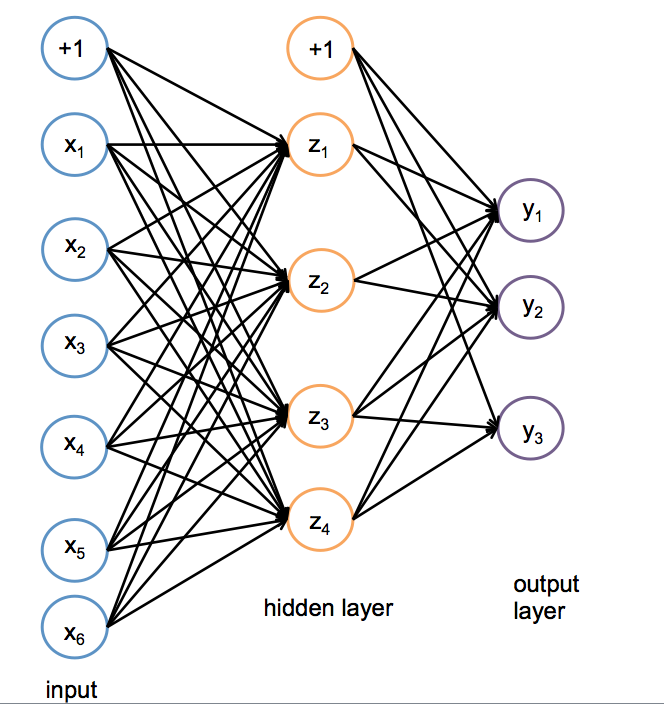
\includegraphics[scale=0.8]{img/oneHL6.png}
        \caption{A One Hidden Layer Neural Network}
        \label{fig:oneHL}
    \end{figure}

\paragraph{Network Overview}
Consider the neural network with one hidden layer shown in Figure \ref{fig:oneHL}. The input layer consists of 6 features $\xv = [x_1,...,x_6]^T$, the hidden layer has 4  nodes $\zv = [z_1,...,z_4]^T$, and the output layer is a probability distribution $\yv = [y_1, y_2, y_3]^T$ over 3 classes. We also add a bias to the input, $x_0 = 1$ and the hidden layer $z_0 = 1$, both of which are fixed to $1$.

$\boldsymbol{\alpha}$ is the matrix of weights from the inputs to the hidden layer and $\boldsymbol{\beta}$ is the matrix of weights from the hidden layer to the output layer. 
$\alpha_{j,i}$ represents the weight going \textit{to} the node $z_j$ in the hidden layer \textit{from} the node $x_i$ in the input layer (e.g. $\alpha_{1,2}$ is the weight from $x_2$ to $z_1$), and $\boldsymbol{\beta}$ is defined similarly. We will use a sigmoid activation function for the hidden layer and a softmax for the output layer. 

\paragraph{Network Details}

Equivalently, we define each of the following. 

The input:

\begin{align}
\xv=[x_1,x_2,x_3,x_4,x_5,x_6]^T
\end{align}

Linear combination at the first (hidden) layer:
\begin{equation}
a_j= \alpha_{j,0} + \sum_{i=1}^6 \alpha_{j,i}*x_i,\,\, \forall j \in \{1,\ldots,4\}
\end{equation}

Activation at the first (hidden) layer:
\begin{align}
z_j &= \sigma(a_j) = \frac{1}{1+\exp(-a_j)},\,\, \forall j \in \{1,\ldots,4\}
\end{align}

Linear combination at the second (output) layer:
\begin{equation}
b_k = \beta_{k,0} + \sum_{j=1}^4 \beta_{k,j}*z_j,\,\, \forall k \in \{1,\ldots,3\}
\end{equation}

Activation at the second (output) layer:
\begin{equation}
\hat{y}_k = \frac{\exp(b_k)}{\sum\limits_{l=1}^3 \exp(b_l)},\,\, \forall k \in \{1,\ldots,3\}
\end{equation}

Note that the linear combination equations can be written equivalently as the product of the weight matrix with the input vector. We can even fold in the bias term $\alpha_0$ by thinking of $x_0 = 1$, and fold in $\beta_{j,0}$ by thinking of $z_0 = 1$.

\paragraph{Loss}

We will use cross entropy loss, $\ell(\hat{\yv},\yv)$. If $\yv$ represents our target output, which will be a one-hot vector representing the correct class, and $\hat{\yv}$ represents the output of the network, the loss is calculated by:
\begin{equation}
   \ell(\hat{\yv},\yv) = - \sum_{i=1}^3 y_i \log(\hat{y}_i)
\end{equation}
For the below questions use natural log in the equation.

\paragraph{Prediction}
When doing prediction, we will predict the $\argmax$ of the output layer. For example, if $\hat{y}_1=0.3, \hat{y}_2=0.2, \hat{y}_3=0.5$ we would predict class 3. If the true class from the training data was $2$ we would have a one-hot vector $\yv$ with values $y_1=0$, $y_2=1$, $y_3=0$.
    
\begin{enumerate}

	\item (6 points) In the following questions you will derive the matrix and vector forms of the previous equations which define out neural network. These are what you should hope to program in order to keep your program under the Autolab time-out.\\
	When working these out it is important to keep a note of the vector and matrix dimensions in order for you to easily identify what is and isn't a valid multiplication. Suppose you are given an training example: $\xv^{(1)}=[x_1,x_2,x_3,x_4,x_5,x_6]^T$ with \textbf{label class 2}, so $\yv^{(1)}=[0,1,0]^T$. We initialize the network weights as:
	\begin{center}
	$$\boldsymbol{\alpha^*}=
	    \begin{bmatrix}
	    \alpha_{1,1} & \alpha_{1,2} & \alpha_{1,3} & \alpha_{1,4} & \alpha_{1,5} & \alpha_{1,6} \\
	    \alpha_{2,1} & \alpha_{2,2} & \alpha_{2,3} & \alpha_{2,4} & \alpha_{2,5} & \alpha_{2,6} \\
	    \alpha_{3,1} & \alpha_{3,2} & \alpha_{3,3} & \alpha_{3,4} & \alpha_{3,5} & \alpha_{3,6} \\
	    \alpha_{4,1} & \alpha_{4,2} & \alpha_{4,3} & \alpha_{4,4} & \alpha_{4,5} & \alpha_{4,6}
	    \end{bmatrix}$$
	    
	$$\boldsymbol{\beta^*}=
	    \begin{bmatrix}
	    \beta_{1,1} & \beta_{1,2} & \beta_{1,3} & \beta_{1,4} \\
	    \beta_{2,1} & \beta_{2,2} & \beta_{2,3} & \beta_{2,4} \\
	    \beta_{3,1} & \beta_{3,2} & \beta_{3,3} & \beta_{3,4}
	    \end{bmatrix}
	$$
	\end{center}
	    
	We want to also consider the bias term and the weights on the bias terms (${\alpha}_{j,0}$ and ${\beta}_{k,0})$. To account for these we can add a new column to the beginning of our initial weight matrices. 
	
	$$\boldsymbol{\alpha}=
	    \begin{bmatrix}
	    \textcolor{blue}{\alpha_{1,0}} & \alpha_{1,1} & \alpha_{1,2} & \alpha_{1,3} & \alpha_{1,4} & \alpha_{1,5} & \alpha_{1,6} \\
	    \textcolor{blue}{\alpha_{2,0}} & \alpha_{2,1} & \alpha_{2,2} & \alpha_{2,3} & \alpha_{2,4} & \alpha_{2,5} & \alpha_{2,6} \\
	    \textcolor{blue}{\alpha_{3,0}} & \alpha_{3,1} & \alpha_{3,2} & \alpha_{3,3} & \alpha_{3,4} & \alpha_{3,5} & \alpha_{3,6} \\
	    \textcolor{blue}{\alpha_{4,0}} & \alpha_{4,1} & \alpha_{4,2} & \alpha_{4,0} & \alpha_{4,4} & \alpha_{4,5} & \alpha_{4,6}
	    \end{bmatrix}$$
	    
	$$\boldsymbol{\beta}=
	    \begin{bmatrix}
	    \textcolor{blue}{\beta_{1,0}} & \beta_{1,1} & \beta_{1,2} & \beta_{1,3} & \beta_{1,4} \\
	    \textcolor{blue}{\beta_{2,0}} & \beta_{2,1} & \beta_{2,2} & \beta_{2,3} & \beta_{2,4} \\
	    \textcolor{blue}{\beta_{3,0}} & \beta_{3,1} & \beta_{3,2} & \beta_{3,3} & \beta_{3,4}
	    \end{bmatrix}$$
	
	    And we can set our first value of our input vectors to always be 1 ($x_0^{(i)} = 1$), so our input becomes: $$\xv^{(1)}=[\textcolor{blue}{1},x_1,x_2,x_3,x_4,x_5,x_6]^T$$
	    
	    
	    \begin{questions}
	        \question[1] By examining the shapes of the initial weight matrices, how many neurons do we have in the first hidden layer of the neural network? (Not including the bias neuron)
	        
	        \begin{tcolorbox}[fit,height=1cm, width=2cm, blank, borderline={1pt}{-2pt}]
	            %solution 
	        \end{tcolorbox}
	        
	        
	        
	        
	        \question[1] How many output neurons will our neural network have?
	        
	        \begin{tcolorbox}[fit,height=1cm, width=2cm, blank, borderline={1pt}{-2pt}]
	            %solution 
	        \end{tcolorbox}
	        
	        
	        
	        
	        \question[1] What is the vector $\av$ whose elements are made up of the entries $a_j$ in equation (1.2). Write your answer in terms of $\alpha$ and $x^{(1)}$.
	        
	        \begin{tcolorbox}[fit,height=1cm, width=4cm, blank, borderline={1pt}{-2pt}]
	            %solution 
	        \end{tcolorbox}
	        
	        
	        
	        
	        \question[1] What is the vector $\zv$ whose elements are made up of the entries $z_j$ in equation (1.3)? Write your answer in terms of $\av$.
	        
	        \begin{tcolorbox}[fit,height=1cm, width=4cm, blank, borderline={1pt}{-2pt}]
	            %solution 
	        \end{tcolorbox}
	        
	        \clearpage	        

	        \question[1] \textbf{Select one:} We cannot take the matrix multiplication of our weights $\beta$ and our vector $\zv$ since they are not compatible shapes. Which of the following would allow us to take the matrix multiplication of $\beta$ and $\zv$ such that the entries of the vector $\bv = \beta*\zv$ are equivalent to the values of $b_k$ in equation (1.4)? 
	        
	        \begin{checkboxes}{}
	        \choice Remove the last column of $\beta$
	        \choice Remove the first row of $\zv$
	        \choice Append a value of 1 to be the first entry of $\zv$
	        \choice Append an additional column of 1's to be the first column of $\beta$ 
	        \choice Append a row of 1's to be the first row of $\beta$ 
	        \choice Take the transpose of $\beta$
	        \end{checkboxes}
	        
	        
	        
	        
	        \question[1] What are the entries of the output vector $\hat{\yv}$? Your answer should be written in terms of $b_1,b_2,b_3$.
	        
	        \begin{tcolorbox}[fit,height=4cm, width=15cm, blank, borderline={1pt}{-2pt}]
	            %solution 
	        \end{tcolorbox}
	        
	        
	        
	    \end{questions} 
	
	\item (12 points) We will now derive the matrix and vector forms for the backpropagation algorithm.
	
	$$\frac{d\ell}{d\alphav} = 
	    \begin{bmatrix}
	        \adj{\alpha_{10}} & \adj{\alpha_{11}} & \dots  & \adj{\alpha_{1M}} \\
	        \adj{\alpha_{20}} & \adj{\alpha_{21}} & \dots  & \adj{\alpha_{2M}} \\
	        \vdots      & \vdots      & \ddots & \vdots \\
	        \adj{\alpha_{D0}} & \adj{\alpha_{D1}} & \dots  & \adj{\alpha_{DM}}
	    \end{bmatrix}$$
	
	
	
	
	The mathematics which you have to derive in this section jump significantly in difficultly, you should always be examining the shape of the matrices and vectors and making sure that you are comparing your matrix elements with calculations of individual derivatives to make sure they match (e.g. the element of the matrix $(\frac{d\ell}{d\alpha})_{2,1}$ should be equal to $\frac{d\ell}{d\alpha_{2,1}}$  ). Recall that $\ell$ is our loss function defined in equation (1.6)
	    
	    \begin{questions}
	        \question[3] The derivative of the softmax function with respect to $b_k$ is as follows:
	        $$\frac{d\hat{y}_l}{db_k} = \hat{y}_l(\Ib[k=l]-\hat{y}_k)$$ 
	        where $\Ib[k=l]$ is an indicator function such that if $k=l$ then it it returns value 1 and 0 otherwise. 
	        Using this, write the derivative $\frac{d\ell}{db_k}$ in a smart way such that you do not need this indicator function? Write your solutions in terms of $\hat{\yv},\yv$.
	        
	        
	        \begin{tcolorbox}[fit,height=1cm, width=6cm, blank, borderline={1pt}{-2pt}]
	            %solution 
	        \end{tcolorbox}
	        
	        
	        \question[2] What are the elements of the vector $\frac{d\ell}{db}$? (Recall that  $\yv^{(1)}=[0,1,0]^T$)
	        
	        
	        \begin{tcolorbox}[fit,height=1cm, width=6cm, blank, borderline={1pt}{-2pt}]
	            %solution 
	        \end{tcolorbox}
	        
	        
	        
	        \question[1] What is the derivative $\frac{d\ell}{d\beta}$? Your answer should be in terms of $\frac{d\ell}{d\bv}$ and $\zv$.
	        
	        
	        \begin{tcolorbox}[fit,height=3cm, width=6cm, blank, borderline={1pt}{-2pt}]
	            %solution 
	        \end{tcolorbox}
	        
	        
	        
	        
	        \question[1] Explain in one short sentance why must we gok back to using the matrix $\betav^*$ (The matrix $\betav$ without the first column of ones) when calculating the matrix $\frac{d\ell}{d\alpha}$?
	        
	        
	        \begin{tcolorbox}[fit,height=1cm, width=15cm, blank, borderline={1pt}{-2pt}]
	            %solution 
	        \end{tcolorbox}
	        
	        
	        
	        
	        \question[1] What is the derivative $\frac{d\ell}{d\zv}$? Your answer should be in terms of $\frac{d\ell}{d\bv}$ and $\betav^*$
	        
	        
	        \begin{tcolorbox}[fit,height=3cm, width=6cm, blank, borderline={1pt}{-2pt}]
	            %solution 
	        \end{tcolorbox}
	        
	        
	        
	        
	        \question[3] What is the derivative $\frac{d\ell}{d\av}$ in terms of $\frac{d\ell}{d\zv}$ and $\zv$
	        
	        
	        \begin{tcolorbox}[fit,height=3cm, width=6cm, blank, borderline={1pt}{-2pt}]
	            %solution 
	        \end{tcolorbox}
	        
	        
	        
	        \question[1] What is the matrix $\frac{d\ell}{d\alpha}$? Your answer should be in terms of $\frac{d\ell}{d\av}$ and $x^{(1)}$.
	        
	        
	        \begin{tcolorbox}[fit,height=3cm, width=6cm, blank, borderline={1pt}{-2pt}]
	            %solution 
	        \end{tcolorbox}
	        
	    \end{questions}
	
	    
	
	\item (9 points) Now you will put these equations to use in an example with numerical values. \textbf{You should use the answers you get here to debug your code.} \\
	You are given a training example $\xv^{(1)}=[1,1,0,0,1,1]^T$ with \textbf{label class 2}, so $\yv^{(1)}=[0,1,0]^T$. We initialize the network weights as:
	\begin{center}
	$$\boldsymbol{\alpha^*}=
	    \begin{bmatrix}
	    1 & 2 & -3 & 0 & 1 & -3 \\
	    3 & 1 & 2 & 1 & 0 & 2 \\
	    2 & 2 & 2 & 2 & 2 & 1 \\
	    1 & 0 & 2 & 1 & -2 & 2
	    \end{bmatrix}$$
	    
	$$\boldsymbol{\beta^*}=
	    \begin{bmatrix}
	    1 & 2 & -2 & 1 \\
	    1 & -1 & 1 & 2 \\
	    3 & 1 & -1 & 1
	    \end{bmatrix}
	$$
	\end{center}
	    
	We want to also consider the bias term and the weights on the bias terms (${\alpha}_{j,0}$ and ${\beta}_{j,0})$. Lets say they are all initialized to 1. To account for this we can add a column of 1's to the beginning of our initial weight matrices. 
	
	$$\boldsymbol{\alpha}=
	    \begin{bmatrix}
	    \textcolor{blue}{1} & 1 & 2 & -3 & 0 & 1 & -3 \\
	    \textcolor{blue}{1} & 3 & 1 & 2 & 1 & 0 & 2 \\
	    \textcolor{blue}{1} & 2 & 2 & 2 & 2 & 2 & 1 \\
	    \textcolor{blue}{1} & 1 & 0 & 2 & 1 & -2 & 2
	    \end{bmatrix}$$
	    
	$$\boldsymbol{\beta}=
	    \begin{bmatrix}
	    \textcolor{blue}{1} & 1 & 2 & -2 & 1 \\
	    \textcolor{blue}{1} & 1 & -1 & 1 & 2 \\
	    \textcolor{blue}{1} & 3 & 1 & -1 & 1
	    \end{bmatrix}
	$$
	
	    And we can set our first value of our input vectors to always be 1 ($x_0^{(i)} = 1$), so our input becomes: $$\xv^{(1)}=[\textcolor{blue}{1},1,1,0,0,1,1]^T$$
	    
	     Using the initial weights, run the feed forward of the network over this example (rounding to 4 decimal places during the calculation) and then answer the following questions. 
	    %In your responses, round to four decimal places---if the answer is an integer you need not include trailing zeros. 
	    % NOT NEEDED: (Note: the superscript $(1)$ simply indicates that a value corresponds to using training example $x^{(1)}$)
	    
	    \begin{questions}
	        \question[1] What is $a_1$?
	        
	        \begin{tcolorbox}[fit,height=1cm, width=2cm, blank, borderline={1pt}{-2pt}]
	            %solution 
	        \end{tcolorbox}
	        
	        
	        \question[1] What is $a_2$?
	        
	        \begin{tcolorbox}[fit,height=1cm, width=2cm, blank, borderline={1pt}{-2pt}]
	            %solution 
	        \end{tcolorbox}
	        
	        
	        
	        \question[1] What is $z_1$?
	        
	        \begin{tcolorbox}[fit,height=1cm, width=2cm, blank, borderline={1pt}{-2pt}]
	            %solution 
	        \end{tcolorbox}
	        
	        
	        \question[1] What is $z_3$?
	        
	        \begin{tcolorbox}[fit,height=1cm, width=2cm, blank, borderline={1pt}{-2pt}]
	            %solution 
	        \end{tcolorbox}
	        
	        
	        
	        \question[1] What is $b_1$?
	        
	        \begin{tcolorbox}[fit,height=1cm, width=2cm, blank, borderline={1pt}{-2pt}]
	            %solution 
	        \end{tcolorbox}
	        
	        
	        \question[1] What is $b_2$?
	        
	        \begin{tcolorbox}[fit,height=1cm, width=2cm, blank, borderline={1pt}{-2pt}]
	            %solution 
	        \end{tcolorbox}
	        
	        
	        
	        \question[1] What is $\hat{y}_2$?
	        
	        \begin{tcolorbox}[fit,height=1cm, width=2cm, blank, borderline={1pt}{-2pt}]
	            %solution 
	        \end{tcolorbox}
	        
	        
	        \question[1] Which class would we predict on this example? Your answer should just be an integer.
	        
	        \begin{tcolorbox}[fit,height=1cm, width=2cm, blank, borderline={1pt}{-2pt}]
	            %solution 
	        \end{tcolorbox}
	        
	        
	        \question[1] What is the total loss on this example?
	        
	        \begin{tcolorbox}[fit,height=1cm, width=2cm, blank, borderline={1pt}{-2pt}]
	            %solution 
	        \end{tcolorbox}
	        
	    \end{questions}
	    
	    \clearpage
	\item (7 points) Now use the results of the previous question to run backpropagation over the network and update the weights. Use learning rate $\eta=1$. 
	    
	    Do your backpropagation calculations rounding to 4 decimal places then answer the following questions: 
	    
	     \begin{questions}
	        \question[1] What is the value of $\frac{d\ell}{d\beta_{1,0}}$?
	        
	        \begin{tcolorbox}[fit,height=1cm, width=2cm, blank, borderline={1pt}{-2pt}]
	            %solution 
	        \end{tcolorbox}
	        
	     
	     
	        \question[1] What is the updated value of the weight $\beta_{1,0}$?
	        
	        \begin{tcolorbox}[fit,height=1cm, width=2cm, blank, borderline={1pt}{-2pt}]
	            %solution 
	        \end{tcolorbox}
	        
	        
	        \question[2] What is the updated value of the weight ${\alpha}_{3,4}$?
	        
	        \begin{tcolorbox}[fit,height=1cm, width=2cm, blank, borderline={1pt}{-2pt}]
	            %solution 
	        \end{tcolorbox}
	        
	        
	        \question[2] What is the updated weight of the input layer bias term applied to $z_2$ (i.e. ${\alpha}_{2,0}$)?
	        
	        \begin{tcolorbox}[fit,height=1cm, width=2cm, blank, borderline={1pt}{-2pt}]
	            %solution 
	        \end{tcolorbox}
	        
	        
	        \question[1] If we ran backpropagation on this example for a large number of iterations and then ran feed forward over the same example again, which class would we predict?
	        
	        \begin{tcolorbox}[fit,height=1cm, width=2cm, blank, borderline={1pt}{-2pt}]
	            %solution 
	        \end{tcolorbox}
	        
	
	    \end{questions}
	
	
	    
	
	 

\end{enumerate}
\clearpage
\subsection{Empirical Questions [10 points]}
\label{sec:interp}

The following questions should be completed after you work through the programming portion of this assignment (Section \ref{sec:code}).

For these questions, \textbf{use the large dataset}.

Use the following values for the hyperparameters unless otherwise specified:

\begin{table}[H]
    \centering
    \begin{tabular}{|c|c|}
        \hline
        \textbf{Paramater} & \textbf{Value} \\
        \hline
        Number of Hidden Units & 50 \\
        \hline
        Weight Initialization & {\sc Random} \\
        \hline
        Learning Rate & 0.01 \\
        \hline
        
    \end{tabular}
    \caption{Default values of hyperparameters for experiments in Section \ref{sec:interp}.}
    \label{tab:params}
\end{table}

 For the following questions, submit your solutions to Gradescope. Please submit computer-generated plots for Q4 and Q6. Do {\bf not} include any visualization-related code when submitting to Autolab! Note: we expect it to take about {\bf 5 minutes} to train each of these networks.
 
\begin{questions}
\setcounter{enumi}{4}
\question[4]  %% hidden units
Train a single hidden layer neural network using the hyperparameters mentioned in Table \ref{tab:params}, except for the number of hidden units which should vary among 5, 20, 50, 100, and 200.  Run the optimization for 100 epochs each time.

Plot the average training cross-entropy (sum of the cross-entropy terms over the training dataset divided by the total number of training examples) on the y-axis vs number of hidden units on the x-axis. In the \textbf{same figure}, plot the average \ntset \thinspace cross-entropy.

 \begin{tcolorbox}[fit,height=10cm, width=15cm, blank, borderline={1pt}{-2pt}]
    %solution 
 \end{tcolorbox}



\clearpage
\question[1]
Examine and comment on the the plots of training and \ntset\thinspace cross-entropy. What is the effect of changing the number of hidden units?

 \begin{tcolorbox}[fit,height=8cm, width=15cm, blank, borderline={1pt}{-2pt}]
    %solution 
    \end{tcolorbox}

%How does the network’s performance differ on the training set versus the validation set during learning? Use the plot of error curves (training and validation) to
%support your argument.

%Visualize the output of the second layer after 30 iterations of training. Note that the output of first layer is simply the image itself (because the first layer
%is data layer). The output of the second layer (convolution) is $20$ images, each of size $24 \times 24$, hence $24 \times 24 \times 20$. Show $20$ images from the layer on a single figure file. 



\clearpage
\question[4] %%% different learning rates
Train a single hidden layer neural network using the hyperparameters mentioned in Table \ref{tab:params}, except for the learning rate which should vary among 0.1, 0.01, and 0.001. Run the optimization for 100 epochs each time.

Plot the average training cross-entropy on the y-axis vs the number of epochs on the x-axis for the mentioned learning rates. In the \textbf{same figure}, plot the average \ntset\thinspace cross-entropy loss. For the sake of clarity, please make a separate figure for each learning rate.

 \begin{tcolorbox}[fit,height=18cm, width=15cm, blank, borderline={1pt}{-2pt}]
    %solution 
    \end{tcolorbox}




\clearpage
\question[1] 
Examine and comment on the the plots of training and \ntset\thinspace cross-entropy. How does adjusting the learning rate affect the convergence of cross-entropy of each dataset?

 \begin{tcolorbox}[fit,height=10cm, width=15cm, blank, borderline={1pt}{-2pt}]
    %solution 
    \end{tcolorbox}


\question[0] After you have completed all other components of this assignment, report your answers to the collaboration policy questions detailed in the Academic Integrity Policies found \href{http://www.cs.cmu.edu/~mgormley/courses/10601bd-f18/about.html#7-academic-integrity-policies}{here}.
    \begin{enumerate*}
        \item Did you receive any help whatsoever from anyone in solving this assignment? Is so, include full details.
        \item Did you give any help whatsoever to anyone in solving this assignment? Is so, include full details.
        \item Did you find or come across code that implements any part of this assignment ? If so, include full details.
    \end{enumerate*}

\begin{tcolorbox}[fit,height=8cm, width=15cm, blank, borderline={1pt}{-2pt}]
    %solution 
    \end{tcolorbox}

\end{questions}\clearpage

\section{Programming [75 points]}
\label{sec:code}

\begin{figure}[H]
    \centering
    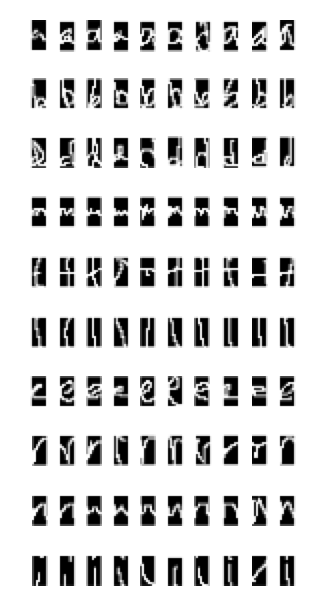
\includegraphics[scale=0.99]{img/10lettergrid.png}
    \caption{10 Random Images of Each of 10 Letters in OCR}
    \label{fig:grid}
\end{figure}

Your goal in this assignment is to label images of handwritten letters by implementing a Neural Network from scratch. You will implement all of the functions needed to initialize, train, evaluate, and make predictions with the network. 
%
The programs you write will be automatically graded using the Autolab system. You may write your programs in \textbf{Octave, Python, Java, or C++}. However, you should use the same language for all parts below. \textbf{Please read the FAQ post on Piazza} before starting the programming portion to ensure that you use correct versions of programming languages/ libraries and do not use any forbidden libraries/ functions!

\subsection{The Task and Datasets}
\label{sec:dataset}

\paragraph{Materials} Download the tar file from Autolab (``Download
  handout"). The tar file will contain all the data that you will need
  in order to complete this assignment.

\paragraph{Datasets} We will be using a subset of an Optical Character Recognition (OCR) dataset. This data includes images of all 26 handwritten letters; our subset will include only the letters ``a," ``e," ``g," ``i," ``l," ``n," ``o," ``r," ``t," and ``u."  The handout contains three datasets drawn from this data: a small dataset with 60 samples per class (50 for training and 10 for \ntset), a medium dataset with 600 samples per class (500 for training and 100 for \ntset), and a large dataset with 1000 samples per class (900 for training and 100 for \ntset). Figure \ref{fig:grid} shows a random sample of 10 images of few letters from the dataset.

\paragraph{File Format} Each dataset (small, medium, and large) consists of two csv files---train and \ntset. Each row contains 129 columns separated by commas. The first column contains the label and columns 2 to 129 represent the pixel values of a $16 \times 8$ image in a row major format. Label 0 corresponds to ``a," 1 to ``e," 2 to ``g," 3 to ``i," 4 to ``l," 5 to ``n," 6 to ``o," 7 to ``r," 8 to ``t," and 9 to ``u."
%
Because the original images are black-and-white (not grayscale), the pixel values are either 0 or 1. However, you should write your code to accept arbitrary pixel values in the range [0,1]. The images in Figure \ref{fig:grid} were produced by converting these pixel values into .png files for visualization. Observe that no feature engineering has been done here; instead the neural network you build will \emph{learn} features appropriate for the task of character recognition.


\subsection{Model Definition}

In this assignment, you will implement a single-hidden-layer neural network with a sigmoid activation function for the hidden layer, and a softmax on the output layer. Let the input vectors $\xv$ be of length $M$, the hidden layer $\zv$ consist of $D$ hidden units, and the output layer $\hat{\yv}$ be a probability distribution over $K$ classes. That is, each element $y_k$ of the output vector represents the probability of $\xv$ belonging to the class $k$. 

\begin{align*}
&  \hat{y}_k = \frac{\exp(b_k)}{\sum_{l=1}^K \exp(b_l)}
\\
& b_k =  \beta_{k,0} + \sum_{j=1}^D \beta_{kj} z_j
\\
& z_j = \frac{1}{1+\exp(-a_j)}
\\
& a_j = \alpha_{j,0} + \sum_{m=1}^M \alpha_{jm} x_m
\end{align*}

We can compactly express this model by assuming that $x_0=1$ is a bias feature on the input and that $z_0=1$ is also fixed. In this way, we have two parameter matrices $\alphav \in \Rb^{D \times (M+1)}$ and $\betav \in \Rb^{K \times (D+1)}$. The extra $0$th column of each matrix (i.e. $\alphav_{\cdot,0}$ and $\betav_{\cdot,0}$) hold the bias parameters.

\begin{align*}
&  \hat{y}_k = \frac{\exp(b_k)}{\sum_{l=1}^K \exp(b_l)}
\\
& b_k =  \sum_{j=0}^D \beta_{kj} z_j
\\
& z_j = \frac{1}{1+\exp(-a_j)}
\\
& a_j = \sum_{m=0}^M \alpha_{jm} x_m
\end{align*}

The objective function we will use for training the neural network is the average cross entropy over the training dataset $\Dc = \{ (\xv^{(i)}, \yv^{(i)}) \}$:

\begin{equation}
\label{eq:celoss}
%\ell(\hat{y},y)=-\sum_{c=1}^M y_{o,c}log(\hat{y}_{o,c})
J(\alphav, \betav)= - \frac{1}{N} \sum_{i=1}^N \sum_{k=1}^{K} y_k^{(i)} \log (\hat{y}^{(i)}_k)
\end{equation}

In Equation~\ref{eq:celoss}, $J$ is a function of the model parameters $\alphav$ and $\betav$ because $\hat{y}^{(i)}_k$ is implicitly a function of $\xv^{(i)}$, $\alphav$, and $\betav$ since it is the output of the neural network applied to $\xv^{(i)}$. Of course, $\hat{y}^{(i)}_k$ and $y_k^{(i)}$ are the $k$th components of $\hat{\yv}^{(i)}$ and $\yv^{(i)}$ respectively.


To train, you should optimize this objective function using stochastic gradient descent (SGD), where the gradient of the parameters for each training example is computed via backpropagation.

\subsubsection{Initialization}
\label{sec:init}

%\item Write your code such that a user can choose to use either 0 or 0.1 for weights initialization. Here the initialization of weights are from a uniform distribution from -r to r where r is 0 or 0.1. Bias terms will always be initialized to 0.

In order to use a deep network, we must first initialize the weights and biases in the network. This is typically done with a random initialization, or initializing the weights from some other training procedure. For this assignment, we will be using two possible initialization: 
\begin{quote}
\begin{description}
\item[{\sc Random}] The weights are initialized randomly from a uniform distribution from -0.1 to 0.1. The bias parameters are initialized to zero.
\item[{\sc Zero}] All weights are initialized to 0.  
\end{description}
\end{quote}

You must support both of these initialization schemes.

%However, for the purpose of this assignment, we will initialize our weights to ============== .
%One way to initialize a neural network is to implement a function which takes input size, number of hidden layers, size of each hidden layer and number of classes as inputs, and return a list of Weights and Biases.



%\subsubsection{Gradient Checker}
%One common way to check
%if the backward pass is correct is by writing a gradient checker. A good %explanation of a gradient checker is in the link: \\
%\href{http://ufldl.stanford.edu/tutorial/supervised/DebuggingGradientChecking/}{http://ufldl.stanford.edu/tutorial/supervised/DebuggingGradientChecking/}


\subsection{Implementation}
\label{sec:model}
Write a program \texttt{neuralnet.\{py|java|cpp|m\}} that implements an optical character recognizer using a one hidden layer neural network with sigmoid activations. Your program should learn the parameters of the model on the training data, report the cross-entropy at the end of each epoch on both train and validation data, and at the end of training write out its predictions and error rates on both datasets. 
%

Your implementation must satisfy the following requirements:
% TODO: Do they need to handle tie breaking in a certain way?
\begin{itemize}
    \item Use a {\bf sigmoid} activation function on the hidden layer and {\bf softmax} on the  output layer to ensure it forms a proper probability distribution.
    \item Number of {\bf hidden units} for the hidden layer should be determined by a command line flag.
    \item Support two different {\bf initialization strategies}, as described in Section \ref{sec:init}, selecting between them via a command line flag.
    \item Use stochastic gradient descent (SGD) to optimize the parameters for one hidden layer neural network. The number of {\bf epochs} will be specified as a command line flag. 
    \item Set the {\bf learning rate} via a command line flag.
    \item Perform stochastic gradient descent updates on the training data in the order that the data is given in the input file. Although you would typically shuffle training examples when using stochastic gradient descent, in order to autograde the assignment, we ask that you {\bf DO NOT} shuffle trials in this assignment.
    \item You may assume that the input data will always have the same \emph{number} of features (i.e. number of columns) and the same output label space (i.e. $\{0,1,\ldots,9\}$). Other than these assumptions, do not hard-code any aspects of the data sets into your code. We will autograde your programs on multiple (hidden) data sets that include different examples.
    \item Do \emph{not} use any machine learning libraries. You may use supported linear algebra packages. See Section \ref{sec:args} for more details.
\end{itemize}

Implementing a neural network can be tricky: the parameters are not just a simple vector, but a collection of many parameters; computational efficiency of the model itself becomes essential; the initialization strategy dramatically impacts overall learning quality;  other aspects which we will \emph{not} change (e.g. activation function, optimization method) also have a large effect. These \emph{tips} should help you along the way:

\begin{itemize}
\item Try to ``vectorize'' your code as much as possible---this is particularly important for Python and Octave. For example, in Python, you want to avoid for-loops and instead rely on \lstinline{numpy} calls to perform operations such as matrix multiplication, transpose, subtraction, etc. over an entire \lstinline{numpy} array at once. Why? Because these operations are actually implemented in fast C code, which won't get bogged down the way a high-level scripting language like Python will.
\item For low level languages such as Java/C++, the use of primitive arrays and for-loops would not pose any computational efficiency problems---however, it is still helpful to make use of a linear algebra library to cut down on the number of lines of code you will write.
\item Implement a finite difference test to check whether your implementation of backpropagation is correctly computing gradients. If you choose to do this, comment out this functionality once your backward pass starts giving correct results and before submitting to Autolab---since it will otherwise slow down your code.
\end{itemize}

\subsubsection{Command Line Arguments}
\label{sec:args}
The autograder runs and evaluates the output from the files generated, using the following command:

\begin{tabular}{ll}
For Python: &
\begin{lstlisting}[language=Shell]
$ python neuralnet.py [args...]
\end{lstlisting}
\\
For Java: &
\begin{lstlisting}[language=Shell]
$ javac -cp "./lib/ejml-v0.33-libs/*:./" neuralnet.java
$ java -cp "./lib/ejml-v0.33-libs/*:./" neuralnet [args...]
\end{lstlisting}
\\
For C++: &
\begin{lstlisting}[language=Shell]
$ g++ -g -std=c++11 -I./lib neuralnet.cpp; ./a.out [args...]
\end{lstlisting}
\\
For Octave: &
\begin{lstlisting}[language=Shell]
$ octave -qH neuralnet.m [args...]
\end{lstlisting}
\end{tabular}

Where above \texttt{[args\dots]} is a placeholder for nine command-line arguments: \texttt{<train\_input>}\newline \texttt{\ntset\_input> <train\_out> <\ntset\_out> <metrics\_out> <num\_epoch> \newline <hidden\_units>  <init\_flag> <learning\_rate>}. These arguments are described in detail below:
\begin{enumerate}
    \item \texttt{<train\_input>}: path to the training input \texttt{.csv} file (see Section~\ref{sec:dataset})
    \item \texttt{<\ntset\_input>}: path to the \ntset \ input \texttt{.csv} file (see Section~\ref{sec:dataset})
    \item \texttt{<train\_out>}: path to output \texttt{.labels} file to which the prediction on the \emph{training} data should be written (see Section~\ref{output})
    \item \texttt{<\ntset\_out>}: path to output \texttt{.labels} file to which the prediction on the \emph{\ntset} data should be written (see Section~\ref{output})
    \item \texttt{<metrics\_out>}: path of the output \texttt{.txt} file to which metrics such as train and \ntset\thinspace error should be written (see Section~\ref{metrics})
    %\item \texttt{<model\_out>}: path of the output \texttt{.txt} file to which the model parameters should be written (see Section~\ref{model})
    \item \texttt{<num\_epoch>}: integer specifying the number of times backpropogation loops through all of the training data (e.g., if \texttt{<num\_epoch>} equals 5, then each training example will be used in backpropogation 5 times).
    \item \texttt{<hidden\_units>}: positive integer specifying the number of hidden units. 
    %(see Section \ref{sec:model} for details)
    %\item \texttt{<activation\_flag>}: integer taking value 1 or 2 that specifies whether to use sigmoid or relu as the activation function (see Section~\ref{sec:model})---that is, if \lstinline{init_flag}==1 use sigmoid; if \lstinline{init_flag}==2 use relu. 
    \item \texttt{<init\_flag>}: integer taking value 1 or 2 that specifies whether to use {\sc Random} or {\sc Zero} initialization (see Section~\ref{sec:init} and Section~\ref{sec:model})---that is, if \lstinline{init_flag}==1 initialize your weights randomly from a uniform distribution over the range [-0.1,0.1] (i.e. {\sc Random}), if \lstinline{init_flag}==2 initialize all weights to zero (i.e. {\sc Zero}). For both settings, {\bf always initialize bias terms to zero}.
    \item \texttt{<learning\_rate>}: float value specifying the learning rate for SGD.
    
\end{enumerate}

As an example, if you implemented your program in Python, the following command line would run your program with 4 hidden units on the small data provided in the handout for 2 epochs using zero initialization and a learning rate of 0.1.
\\
\begin{lstlisting}[language=Shell]
$ python neuralnet.py smallTrain.csv smallTest.csv \ 
model1train_out.labels model1test_out.labels model1metrics_out.txt \ 
2 4 2 0.1
\end{lstlisting}

\begin{notebox}
\paragraph{Linear Algebra Libraries} When implementing a neural network, it is often more convenient to have a linear algebra library at your disposal. In this assignment, Java users may use EJML\footnote{\url{https://ejml.org}} and C++ users Eigen\footnote{\url{http://eigen.tuxfamily.org/}}. Details below. 
%
(As usual, Python users have numpy; Octave users have built-in matrix support.)
%
\begin{description}
\item[Java] EJML is a pure Java linear algebra package with three interfaces. We strongly recommend using the SimpleMatrix interface. Autolab will use EJML version 3.3. The command line arguments above demonstrate how we will call you code. The classpath inclusion \lstinline{-cp "./lib/ejml-v0.33-libs/*:./"} will ensure that all the EJML jars are on the classpath as well as your code. 
\item[C++] Eigen is a header-only library, so there is no linking to worry about---just \lstinline{#include} whatever components you need. Autolab will use Eigen version 3.3.4. The command line arguments above demonstrate how we will call you code. The argument \lstinline{-I./lib} will include the \lstinline{lib/Eigen} subdirectory, which contains all the headers.
\end{description} 
We have included the correct versions of EJML/Eigen in the handout.tar for your convenience. Do {\bf not} include EJML or Eigen in your Autolab submission tar; the autograder will ensure that they are in place. 
\end{notebox}

\subsubsection{Output: Labels Files} \label{output}
Your program should write two output \texttt{.labels} files containing the predictions of your model on training data (\texttt{<train\_out>}) and \ntset\thinspace data (\texttt{<\ntset\_out>}). Each should contain the predicted labels for each example printed on a new line. Use \lstinline{\n} to create a new line. 

Your labels should exactly match those of a reference implementation -- this will be checked by the autograder by running your program and evaluating your output file against the reference solution.

\textbf{Note}: You should output your predicted labels using the same \emph{integer} identifiers as the original training data. You should also insert an empty line (again using ’\textbackslash n’) at the end of each sequence (as is done in the input data files). The first few lines of the predicted labels for the \ntset\thinspace dataset is given below
\\

\begin{lstlisting}
6
4
8
8
\end{lstlisting}


\subsubsection{Output Metrics} \label{metrics}
Generate a file where you report the following metrics: 

\begin{description}
\item[cross entropy] After each Stochastic Gradient Descent (SGD) epoch, report mean cross entropy on the training data \lstinline{crossentropy(train)} and \ntset\thinspace data \texttt{crossentropy(\ntset)} (See Equation~\ref{eq:celoss}). These two cross-entropy values should be reported at the end of each epoch and prefixed by the epoch number. For example, after the second pass through the training examples, these should be prefixed by \lstinline{epoch=2}. The total number of train losses you print out should equal \texttt{num\_epoch}---likewise for the total number of \ntset\thinspace losses.
\item[error] After the final epoch (i.e. when training has completed fully), report the final training error \lstinline{error(train)} and \ntset\thinspace error \texttt{error(\ntset)}. 
\end{description}

%All of your reported numbers should be within 0.01 of the reference solution. 
A sample output is given below. It contains the train and \ntset\thinspace losses for the first 2 epochs and the final error rate when using the command given above.

\begin{lstlisting}
epoch=1 crossentropy(train): 2.18506276114
epoch=1 crossentropy(test): 2.18827302588
epoch=2 crossentropy(train): 1.90103257727
epoch=2 crossentropy(test): 1.91363803461
error(train): 0.77
error(test): 0.78
\end{lstlisting}
%epoch=1 likelihood(train): 1.175428
%epoch=1 likelihood(validation): 1.665414
%epoch=2 likelihood(train): 0.900247
%epoch=2 likelihood(validation): 1.317512
%error(train): 0.314815
%error(test): 0.200000


Take care that your output has the exact same format as shown above. There is an equal sign \lstinline{=} between the word \lstinline{epoch} and the epoch number, but no spaces. There should be a single space after the epoch number (e.g. a space after \lstinline{epoch=1}), and a single space after the colon preceding the metric value (e.g. a space after \lstinline{epoch=1 likelihood(train):}). Each line should be terminated by a Unix line ending \lstinline{\n}.

\subsubsection{Tiny Data Set} \label{tiny}
To help you with this assignment, we have also included a tiny data set, \texttt{tinyTrain.csv} and \texttt{tinyTest.csv}, and a reference output file \texttt{tinyOutput.txt} for you to use. The tiny dataset is in the similar format to the other datasets, but it only contains two samples with five features. The reference file contains outputs from each layer for both the forward and back-propagation steps. We advise you to use this set to help you debug in case your implementation doesn't produce the same results as described in Section 2.3.3.

There is more information in the \texttt{README for students.md} file. Do read through the README file if you plan to use it for debugging. For your reference, \texttt{tinyOutput.txt} is generated from the following command line specifications:

\begin{lstlisting}[language=Shell]
$ python neuralnet.py tinyTrain.csv tinyTest.csv \
tinyTrain_out.labels tinyTest_out.labels tinyMetrics_out.txt 1 4 2 0.1
\end{lstlisting}
The specific output file names are not important, but be sure to keep the other arguments exactly as they are shown above.

\subsection{Gradescope Submission}
You must submit a .zip file containing \texttt{neuralnet.\{py|m|java|cpp\}} to Gradescope. Please do not use any other file name for your implementation. This will cause problems for the autograder to correctly detect and run your code.

Some additional tips: Make sure to read the autograder output carefully. The autograder for Gradescope prints out some additional 
information about the tests that it ran. For this programming assignment we've specially designed some buggy implementations that you might do, and try our best to detect those and give you some more useful feedback in Gradescope's autograder. Make wise use of autograder's output for debugging your code.

\begin{comment}
You must submit a .tar file named {\tt neuralnet.tar} containing \texttt{neuralnet.\{py|m|java|cpp\}}.
You can create that file by running:
\begin{lstlisting}
tar -cvf neuralnet.tar neuralnet.{py|m|java|cpp}
\end{lstlisting}
from the directory containing your code.

Some additional tips: {\bf DO NOT} compress your files; you are just
creating a tarball. Do not use tar \texttt{-czvf}.  {\bf DO NOT} put
the above files in a folder and then tar the folder.  Autolab is case
sensitive, so observe that all your files should be named in {\bf
  lowercase}. You must submit this file to the corresponding homework
link on Autolab. The autograder for Autolab prints out some additional 
information about the tests that it ran. You can view this output by selecting 
 "Handin History" from the menu and then clicking one of the scores you 
 received for a submission. For example on this assignment, among other things, 
 the autograder will print out which language it detects (e.g. Python, Octave, C++, Java). 
 
 \begin{notebox}
  {\bf Python3 Users:} Please include a blank file called python3.txt (case-sensitive) in your tar submission and we will execute your submitted program using Python 3 instead of Python 2.7.
 \end{notebox}
 
  \begin{notebox}
  {\bf C++Users:} When you submit to autolab, make sure that you are calling the Eigen library using the statement \#include $<$Eigen/Dense$>$
 \end{notebox}
\end{comment}

Note: For this assignment, you may make up to 10 submissions to Autolab before the deadline, but only your last submission will be graded.

%\clearpage



\begin{comment}
\subsection*{Collaboration Policy}
\textbf{Reminder: you should submit your answers to collaboration policy questions to Gradescope with the rest of your solutions.}
\begin{enumerate}[Q1]
    \setcounter{enumi}{11}
    \item \textbf{[1 point]}:
    \begin{itemize}
        \item Did you receive any help whatsoever from anyone in solving this assignment? Please answer \textit{yes} or \textit{no}.
        \item If you answered \textit{yes} on the previous question, please give full details below (e.g., \textit{Christopher Nolan} explained to me what is asked in Question 3.4).
    \end{itemize}
    \item \textbf{[1 point]}: 
    \begin{itemize}
        \item Did you give any help whatsoever to anyone in solving this assignment? Please answer \textit{yes} or \textit{no}.
        \item If you answered \textit{yes} on the previous question, please give full details below (e.g., I pointed \textit{Michael Bay} to section 2.3 since he didn't know how to proceed with Question 2).
    \end{itemize}
    \item \textbf{[1 point]}:
    \begin{itemize}
        \item Did you find or come across code that implements any part of this assignment? Please answer \textit{yes} or \textit{no}.
        \item If you answered \textit{yes} on the previous question, please give full details below (book \& page, URL \& location, movies \& scene, etc).
    \end{itemize}
\end{enumerate}
\end{comment}



\clearpage
\appendix
\section{Implementation Details for Neural Networks}
\label{sec:implementationdetails}

This section provides a variety of suggestions for how to efficiently and succinctly implement a neural network and backpropagation. 

\subsection{SGD for Neural Networks}
\label{sec:sgd}

% $\hat{\yv} = h_{\alphav, \betav}(\xv) = \text{softmax}(\betav \sigma(\alphav \xv + \alphav_0) + \betav_0)$

Consider the neural network described in Section \ref{sec:model} applied to the $i$th training example $(\xv, \yv)$ where $\yv$ is a one-hot encoding of the true label. Our neural network outputs $\hat{\yv} = h_{\alphav, \betav}(\xv)$, where $\alphav$ and $\betav$ are the parameters of the first and second layers respectively and $h_{\alphav, \betav}(\cdot)$ is a one-hidden layer neural network with a sigmoid activation and softmax output. The loss function is negative cross-entropy $J = \ell(\hat{\yv}, \yv) = - \yv^T \log(\hat{\yv})$. $J = J_{\xv, \yv}(\alphav, \betav)$ is actually a function of our training example ($\xv, \yv$), and our model parameters $\alphav, \betav$ though we write just $J$ for brevity.

In order to train our neural network, we are going to apply stochastic gradient descent. Because we want the behavior of your program to be deterministic for testing on Autolab, we make a few simplifications: (1) you should \emph{not} shuffle your data and (2) you will use a fixed learning rate. In the real world, you would \emph{not} make these simplifications. 

SGD proceeds as follows, where $E$ is the number of epochs and $\gamma$ is the learning rate.


\begin{algorithm}[H]
  \caption{Stochastic Gradient Descent (SGD) without Shuffle}
  \label{alg:sgd}
  \begin{algorithmic}[1] % The number tells where the line numbering should start
    \Procedure{SGD}{Training data $\Dc$, \ntset\thinspace data $\Dc_t$} 
      \State Initialize parameters $\alphav, \betav$ \Comment{Use either {\sc Random} or {\sc Zero} from Section \ref{sec:init}}
      \For{$e \in \{1, 2, \ldots, E\}$} \Comment{For each epoch}
        \For{$(\xv, \yv) \in \Dc$} \Comment{For each training example (No shuffling)}
          \State Compute neural network layers:
          %$\hat{\yv} = h_{\alphav, \betav}(\xv)$ and loss $J = \ell(\hat{\yv}, \yv)$ storing intermediate quantities as in 
          \State $\ov = \texttt{object}( \xv, \av, \bv, \zv, \hat{\yv}, J) = \textproc{NNForward}(\xv, \yv, \alphav, \betav)$
          \State Compute gradients via backprop: 
            %    $\nabla_{\alphav} J, \nabla_{\betav} J$
          %\State $\gv_{\alphav} = \nabla_{\alphav} J$
          %\State $\gv_{\betav} = \nabla_{\betav} J$ 
          \State 
              $
                \begin{drcases}
                \gv_{\alphav} = \nabla_{\alphav} J \\
                \gv_{\betav} = \nabla_{\betav} J
                \end{drcases} 
                = \textproc{NNBackward}(\xv, \yv, \alphav, \betav, \ov)
              $
          \State Update parameters:
          \State $\alphav \gets \alphav - \gamma \gv_{\alphav}$
          \State $\betav \gets \betav - \gamma \gv_{\betav}$
            %   \State Update parameters:
            %   \State $\alphav \gets \alphav - \gamma \nabla_{\alphav} J$ 
            %   \State $\betav \gets \betav - \gamma \nabla_{\betav} J$ 
        \EndFor
        \State Evaluate training mean cross-entropy $J_{\Dc}(\alphav, \betav)$
        \State Evaluate \ntset\thinspace mean cross-entropy $J_{\Dc_t}(\alphav, \betav)$
      \EndFor
      \State \textbf{return} parameters $\alphav, \betav$
    \EndProcedure
  \end{algorithmic}
\end{algorithm}
  
%
At test time, we output the most likely prediction for each example: 

\begin{algorithm}[H]
  \caption{Prediction at Test Time}
  \label{alg:predict}
  \begin{algorithmic}[1] % The number tells where the line numbering should start
    \Procedure{Predict}{Unlabeled train or \ntset\thinspace dataset $\Dc'$, Parameters $\alphav, \betav$} 
    \For{$\xv \in \Dc'$}
      \State Compute neural network prediction $\hat{\yv} = h(\xv)$
      \State Predict the label with highest probability $l = \argmax_k \hat{y}_k$
    \EndFor
    \EndProcedure
  \end{algorithmic}
\end{algorithm}

The gradients we need above are themselves matrices of partial derivatives. Let $M$ be the number of input features, $D$ the number of hidden units, and $K$ the number of outputs.

\begin{align}
    &\alphav =
    \begin{bmatrix}
        \alpha_{10} & \alpha_{11} & \dots  & \alpha_{1M} \\
        \alpha_{20} & \alpha_{21} & \dots  & \alpha_{2M} \\
        \vdots      & \vdots      & \ddots & \vdots \\
        \alpha_{D0} & \alpha_{D1} & \dots  & \alpha_{DM}
    \end{bmatrix}
    &&
    \gv_{\alphav} = \nabla_{\alphav} J = 
    \begin{bmatrix}
        \adj{\alpha_{10}} & \adj{\alpha_{11}} & \dots  & \adj{\alpha_{1M}} \\
        \adj{\alpha_{20}} & \adj{\alpha_{21}} & \dots  & \adj{\alpha_{2M}} \\
        \vdots      & \vdots      & \ddots & \vdots \\
        \adj{\alpha_{D0}} & \adj{\alpha_{D1}} & \dots  & \adj{\alpha_{DM}}
    \end{bmatrix}
\end{align}

\begin{align}
    &\betav =
    \begin{bmatrix}
        \beta_{10} & \beta_{11} & \dots  & \beta_{1D} \\
        \beta_{20} & \beta_{21} & \dots  & \beta_{2D} \\
        \vdots      & \vdots      & \ddots & \vdots \\
        \beta_{K0} & \beta_{K1} & \dots  & \beta_{KD}
    \end{bmatrix}
    &&
    \gv_{\betav} = \nabla_{\betav} J = 
    \begin{bmatrix}
        \adj{\beta_{10}} & \adj{\beta_{11}} & \dots  & \adj{\beta_{1D}} \\
        \adj{\beta_{20}} & \adj{\beta_{21}} & \dots  & \adj{\beta_{2D}} \\
        \vdots      & \vdots      & \ddots & \vdots \\
        \adj{\beta_{K0}} & \adj{\beta_{K1}} & \dots  & \adj{\beta_{KD}}
    \end{bmatrix}
\end{align}

Observe that we have (in a rather \emph{tricky} fashion) defined the matrices such that both $\alphav$ and $\gv_{\alphav}$ are $D \times (M+1)$ matrices. Likewise, $\betav$ and $\gv_{\betav}$ are $K \times (D+1)$ matrices. The $+1$ comes from the extra columns $\alphav_{\cdot, 0}$ and $\betav_{\cdot, 0}$ which are the bias parameters for the first and second layer respectively. We will always assume $x_0 = 1$ and $z_0 = 1$. This should greatly simplify your implementation as you will see in Section \ref{sec:vectorize}.


\subsection{Recursive Derivation of Backpropagation}
\label{sec:recursive}

In class, we described a very general approach to differentiating arbitrary functions: backpropagation. One way to understand \emph{how} we go about deriving the backpropagation algorithm is to consider the natural consequence of recursive application of the chain rule. 

In practice, the partial derivatives that we need for learning are $\adj{\alpha_{ij}}$ and $\adj{\beta_{kj}}$.

\subsubsection{Symbolic Differentiation}

\begin{notebox}
\paragraph{Note} In this section, we motivate backpropagation via a strawman: that is, we will work through the \emph{wrong} approach first (i.e. symbolic differentiation) in order to see why we want a more efficient method (i.e. backpropagation). Do {\bf not} use this symbolic differentiation in your code.
\end{notebox}

Suppose we wanted to find $\adj{\alpha_{ij}}$ using the method we know from high school calculus. That is, we will analytically solve for an equation representing that quantity.

\begin{enumerate}
    \item Considering the computational graph for the neural network, we observe that $\alpha_{ij}$ has exactly one child $a_j = \sum_{m=0}^M \alpha_{jm} x_m$. That is $a_j$ is the \emph{first and only} intermediate quantity that uses $\alpha_{ij}$. Applying the chain rule, we obtain 
        \[ \chain{a_i}{\alpha_{ij}} = \adj{a_i} x_j \] 
    \item So far so good, now we just need to compute $\adj{a_j}$. Not a problem! We can just apply the chain rule again. $a_j$ just has exactly one child as well, namely $z_j = \sigma(a_j)$. The chain rule gives us that $\chain{z_j}{a_j} = \adj{z_j} z_j (1 - z_j)$. Substituting back into the equation above we find that 
        \[ \adj{\alpha_{ij}} = \adj{z_j} (z_j (1-z_j)) x_i \]
    \item How do we get $\adj{z_j}$? You guessed it: apply the chain rule yet again. This time, however, there are \emph{multiple} children of $z_j$ in the computation graph; they are $b_1, b_2, \ldots b_K$. Applying the chain rule gives us that $\adj{z_j} = \sum_{k=1}^K \adj{b_k}\frac{d b_k}{d z_j} = \sum_{k=1}^K \adj{b_k}\beta_{kj}$. Substituting back into the equation above gives:
        \[ \adj{\alpha_{ij}} = \sum_{k=1}^K \adj{b_k}\beta_{kj} (z_j (1-z_j)) x_i \]
    \item Next we need $\adj{b_k}$, which we again obtain via the chain rule: $\adj{b_k} = \sum_{l=1}^K \adj{\hat{y}_l} \frac{d \hat{y}_l}{d b_k} = \sum_{l=1}^K \adj{\hat{y}_l} \hat{y}_l (\Ib[k=l] - \hat{y}_k)$. Substituting back in above gives:
        \[ \adj{\alpha_{ij}} = \sum_{k=1}^K \sum_{l=1}^K \adj{\hat{y}_l} \hat{y}_l (\Ib[k=l] - \hat{y}_k) \beta_{kj} (z_j (1-z_j)) x_i \]
    \item Finally, we know that $\adj{\hat{y}_l} = - \frac{y_l}{\hat{y}_l}$ which we can again substitute back in to obtain our final result:
        \[ \adj{\alpha_{ij}} = \sum_{k=1}^K \sum_{l=1}^K - \frac{y_l}{\hat{y}_l} \hat{y}_l (\Ib[k=l] - \hat{y}_k) \beta_{kj} (z_j (1-z_j)) x_i \]
    Although we have successfully derived the partial derivative w.r.t. $\alpha_{ij}$, the result is far from satisfying. It is overly complicated and requires deeply nested for-loops to compute.
\end{enumerate}

The above is an example of {\bf symbolic differentiation}. That is, at the end we get an equation representing the partial derivative w.r.t. $\alpha_{ij}$. At this point, you should be saying to yourself: What a mess! Isn't there a better way? Indeed there is and its called backpropagation. The algorithm works just like the above symbolic differentiation except that we \textit{never} subsitute the partial derivative from the previous step back in. Instead, we work ``backwards'' through the steps above computing partial derivatives in a top-down fashion. 

\subsection{Matrix / Vector Operations for Neural Networks}
\label{sec:vectorize}

Some programming languages are fast and some are slow. Below is a simple benchmark to show this concretely. The task is to compute a dot-product $\av^T \bv$ between two vectors $\av \in \Rb^{500}$ and $\bv \in \Rb^{500}$ one thousand times. Table \ref{tab:dotprod} shows the time taken for several combinations of programming language and data structure. 

\begin{table}[H]
    \begin{center}
    \begin{tabular}{llr}
        \toprule
        {\bf language} & {\bf data structure} & {\bf time (ms)} \\
        \midrule
        Python & list & 200.99 \\
        Python & \texttt{numpy} array & 1.01\\
        Java & \texttt{float[]} & 4.00 \\
        C++ & \texttt{vector<float>} & 0.81\\
        \bottomrule
    \end{tabular}
    \end{center}
    \caption{Computation time required for dot-product in various languages.}
    \label{tab:dotprod}
\end{table}

Notice that Java\footnote{Java would approach the speed of C++ if we had given the just-in-time (JIT) compiler inside the JVM time to ``warm-up''.} and C++ with standard data structures are quite efficient. By contrast, Python differs dramatically depending on which data structure you use: with a standard list object \\(e.g. \lstinline{a = [float(i) for x in range(500)]}) the computation time is an appallingly slow 200+ milliseconds. Simply by switching to a numpy array (e.g. \lstinline{a = np.arange(500, dtype=float)}) we obtain a 200x speedup. This is because a numpy array is actually carrying out the dot-product computation in pure C, which is just as fast as our C++ benchmark, modulo some Python overhead.

Thus, for this assignment, Java and C++ programmers could easily implement the entire neural network using standard data structures and some for-loops. However, Python or Octave programmers would find that their code is simply too slow if they tried to do the same. As such, particularly for Python and Octave users, one must convert all the deeply nested for-loops into efficient ``vectorized'' math via \lstinline{numpy}. Doing so will ensure efficient code. Java and C++ programmers can also benefit from linear algebra packages since it can cut down on the total number of lines of code you need to write.

\subsection{Procedural Method of Implementation}
\label{sec:procedural}

Perhaps the simplest way to implement a 1-hidden-layer neural network is procedurally. Note that this approach has some drawbacks that we'll discuss below (Section \ref{sec:proceduraldrawbacks}). 

The procedural method: one function computes the outputs of the neural network and all intermediate quantities $\ov = \textproc{NNForward}(\xv, \yv, \alphav, \betav) = \texttt{object}( \xv, \av, \bv, \zv, \hat{\yv}, J)$, where the object is just some struct. Then another function computes the gradients of our parameters $\gv_{\alphav}, \gv_{\betav} = \textproc{NNBackward}(\xv, \yv, \alphav, \betav, \ov)$, where $\ov$ is a data structure that stores all the forward computation.

One must be careful to ensure that functions are vectorized. For example, your Sigmoid function should be able to take a vector input and return a vector output with the Sigmoid function applied to all of its elements. All of these operations should avoid for-loops when working in a high-level language like Python / Octave. We can compute the softmax function in a similar vectorized manner.

\subsubsection{Drawbacks to Procedural Method}
\label{sec:proceduraldrawbacks}

As noted in Section \ref{sec:finitediff}, it is possible to use a finite difference method to check that the backpropagation algorithm is correctly computing the gradient of its corresponding forward computation. We \emph{strongly} encourage you to do this.

There is a big problem however: what if your finite difference check informs you that the gradient is \emph{not} being computed correctly. How will you know \emph{which} part of your \textproc{NNForward}() or \textproc{NNBackward}() functions has a bug? There are two possible solutions here:
\begin{enumerate}
    \item As usual, you can (and should) work through a tiny example dataset on paper. Compute each intermediate quantity and each gradient. Check that your code reproduces each number. The one that does not should indicate where to find the bug.
    \item Replace your procedural implementation with a module-based one (as described in Section \ref{sec:modulebased}) and then run a finite-difference check on \emph{each} layer of the model individually. The finite-difference check that fails should indicate where to find the bug.
\end{enumerate}

Of course, rather than waiting until you have a bug in your procedural implementation, you could jump straight to the module-based version---though it increases the complexity slightly (i.e. more lines of code) it \emph{might} save you some time in the long run.

\subsection{Module-based Method of Implementation}
\label{sec:modulebased}

Module-based automatic differentiation (AD) is a technique that has long been used to develop libraries for deep learning. Dynamic neural network packages are those that allow a specification of the computation graph dynamically at runtime, such as Torch\footnote{\url{http://torch.ch/}}, PyTorch\footnote{\url{http://pytorch.org/}}, and DyNet\footnote{\url{https://dynet.readthedocs.io}}---these all employ module-based AD in the sense that we will describe here.\footnote{Static neural network packages are those that require a static specification of a computation graph which is subsequently compiled into code. Examples include Theano, Tensorflow, and CNTK. These libraries are also module-based but the particular form of implementation is different from the dynamic method we recommend here.}

The key idea behind module-based AD is to componentize the computation of the neural-network into layers. Each layer can be thought of as consolidating numerous nodes in the computation graph (a subset of them) into one \emph{vector-valued} node. Such a vector-valued node should be capable of the following and we call each one a {\bf module}:
\begin{enumerate}
    \item Forward computation of output $\bv = [b_1, \ldots, b_B]$ given input $\av = [a_1, \ldots, a_A]$ via some differentiable function $f$. That is $\bv = f(\av)$. 
    \item Backward computation of the gradient of the input $\gv_{\av} = \nabla_{\av}J = [\adj{a_1}, \ldots, \adj{a_A}]$ given the gradient of output $\gv_{\bv} = \nabla_{\bv}J = [\adj{b_1}, \ldots, \adj{b_B}]$, where $J$ is the final real-valued output of the entire computation graph. This is done via the chain rule $\adj{a_i} = \sum_{j=1}^J \adj{b_j} \frac{d b_j}{d a_i}$ for all $i \in \{1, \ldots, A\}$.
\end{enumerate}

\subsubsection{Module Definitions}

The modules we would define for our neural network would correspond to a Linear layer, a Sigmoid layer, a Softmax layer, and a Cross-Entropy layer. Each module defines a forward function $\bv = \textproc{*Forward}(\av)$, and a backward function $\gv_{\av} = \textproc{*Backward}(\av, \bv, \gv_{\bv})$ method. These methods accept parameters if appropriate. The dimensions $A$ and $B$ are specific to the module such that we have input $\av \in \Rb^A$, output $\bv \in \Rb^B$, gradient of output $\gv_{\av} \triangleq \nabla_{\av}J \in \Rb^A$, and gradient of input $\gv_{\bv} \triangleq \nabla_{\bv}J \in \Rb^B$. We have provided you the pseudocode for the Linear Module as an example.

\begin{description}
    \item[Linear Module] The linear layer has two inputs: a vector $\av$ and parameters $\omega \in \Rb^{B \times A}$. The output $\bv$ is not used by \textproc{LinearBackward}, but we pass it in for consistency of form.
      \begin{algorithmic}[1]
        \Procedure{LinearForward}{$\av$, $\alphav$}
          \State $\bv = \alphav \av$
          \State \textbf{return} $\bv$
        \EndProcedure
        \Procedure{LinearBackward}{$\av$,  $\alpha$, $\bv$, $\gv_{\bv}$}
          \State $\gv_{\alphav} = \gv_{\bv} \av^T$
          \State $\gv_{\av} = \alphav^T \gv_{\bv}$
          \State \textbf{return} $\gv_{\alphav}, \gv_{\av}$
        \EndProcedure
      \end{algorithmic}
\end{description}

It's also quite common to combine the Cross-Entropy and Softmax layers into one. The reason for this is the cancelation of numerous terms that result from the zeros in the cross-entropy backward calculation. (Said trick is \emph{not} required to obtain a sufficiently fast implementation for Autolab.)
%You can read more about this in a detailed writeup from your TAs on Piazza.\footnote{\url{https://piazza.com/class/jar95m88puk3v6?cid=1092}} (Said trick is \emph{not} required to obtain a sufficiently fast implementation for Autolab.)

\subsubsection{Module-based AD for Neural Network}

Using these modules, we can re-define our functions \textproc{NNForward} and \textproc{NNBackward} as follows. 

\begin{algorithm}[H]
  \caption{Forward Computation}
  \label{alg:forwardmodule}
  \begin{algorithmic}[1] % The number tells where the line numbering should start
    \Procedure{NNForward}{Training example ($\xv$, $\yv$), Parameters $\alphav$, $\betav$}
      \State $\av = \textproc{LinearForward}(\xv, \alphav)$
      \State $\zv = \textproc{SigmoidForward}(\av)$
      \State $\bv = \textproc{LinearForward}(\zv, \betav)$
      \State $\hat{\yv} = \textproc{SoftmaxForward}(\bv)$
      \State $J = \textproc{CrossEntropyForward}(\yv, \hat{\yv})$
      \State $\ov = \texttt{object}(\xv, \av, \zv, \bv, \hat{\yv}, J)$
      \State \textbf{return} intermediate quantities $\ov$
    \EndProcedure
  \end{algorithmic}
\end{algorithm}

\begin{algorithm}[H]
  \caption{Backpropagation}
  \label{alg:backpropmodule}
  \begin{algorithmic}[1] % The number tells where the line numbering should start
    \Procedure{NNBackward}{Training example ($\xv$, $\yv$), Parameters $\alphav$, $\betav$, Intermediates $\ov$}
      \State Place intermediate quantities $\xv, \av, \zv, \bv, \hat{\yv}, J$ in $\ov$ in scope
      \State $g_J = \frac{dJ}{dJ} = 1$ \Comment{Base case}
      \State $\gv_{\hat{\yv}} = \textproc{CrossEntropyBackward}(\yv, \hat{\yv}, J, g_J)$
      \State $\gv_{\bv} = \textproc{SoftmaxBackward}(\bv, \hat{\yv}, \gv_{\hat{\yv}})$
      \State $\gv_{\betav}, \gv_{\zv} = \textproc{LinearBackward}(\zv, \bv, \gv_{\bv})$
      \State $\gv_{\av} = \textproc{SigmoidBackward}(\av, \zv, \gv_{\zv})$
      \State $\gv_{\alphav}, \gv_{\xv} = \textproc{LinearBackward}(\xv, \av, \gv_{\av})$ \Comment{We discard $\gv_{\xv}$}
      \State \textbf{return} parameter gradients $\gv_{\alphav}, \gv_{\betav}$
    \EndProcedure
  \end{algorithmic}
\end{algorithm}

Here's the big takeaway: we can actually view these two functions as themselves defining another module! It is a 1-hidden layer neural network module. That is, the cross-entropy of the neural network for a single training example is \emph{itself} a differentiable function and we know how to compute the gradients of its inputs, given the gradients of its outputs. 

\subsection{Testing Backprop with Numerical Differentiation}
\label{sec:finitediff}

Numerical differentiation provides a convenient method for testing
gradients computed by backpropagation. The \emph{centered}
finite difference approximation is:
\begin{align}
\frac{\partial}{\partial \theta_i} J(\vc{\theta}) \approx \frac{\left( J(\vc{\theta} + \epsilon \cdot \vc{d}_i) - J(\vc{\theta} - \epsilon \cdot \vc{d}_i) \right)}{2\epsilon} 
\end{align}
where $\vc{d}_i$ is a 1-hot vector consisting of all zeros except for
the $i$th entry of $\vc{d}_i$, which has value 1.  Unfortunately, in
practice, it suffers from issues of floating point
precision. Therefore, it is typically only appropriate to use this on
small examples with an appropriately chosen $\epsilon$.

In order to apply this technique to test the gradients of your backpropagation implementation, you will need to ensure that your code is appropriately factored. Any of the modules including \textproc{NNForward} and \textproc{NNBackward} could be tested in this way.
%

For example, you could use two functions: \lstinline{forward(x,y,theta)} computes the cross-entropy for a training example. \lstinline{backprop(x,y,theta)} computes the gradient of the cross-entropy for a training example via backpropagation. Finally, \lstinline{finite_diff} as defined below approximates the gradient by the centered finited difference method. The following pseudocode provides an overview of the entire procedure.

\begin{lstlisting}[language=Python]
def finite_diff(x, y, theta):
    epsilon = 1e-5
    grad = zero_vector(theta.length)
    for m in [1, ..., theta.length]:
        d = zero_vector(theta.length)
        d[m] = 1
        v = forward(x, y, theta + epsilon * d)
        v -= forward(x, y, theta - epsilon * d)
        v /= 2*epsilon
        grad[m] = v
        
# Compute the gradient by backpropagation
grad_bp = backprop(x, y, theta)
# Approximate the gradient by the centered finite difference method
grad_fd = finite_diff(x, y, theta)

# Check that the gradients are (nearly) the same
diff = grad_bp - grad_fd  # element-wise difference of two vectors
print l2_norm(diff) # this value should be small (e.g. < 1e-7)
\end{lstlisting}

\subsubsection{Limitations}

This does \emph{not} catch all bugs---the only thing it tells you is whether your backpropagation implementation is correctly computing the gradient for the forward computation. Suppose your \emph{forward} computation is incorrect, e.g. you are always computing the cross-entropy of the wrong label. If your \emph{backpropagation} is also using the same wrong label, then the check above will not expose the bug. Thus, you always want to \emph{separately} test that your forward implementation is correct.

\subsubsection{Finite Difference Checking of Modules}

Note that the above would test the gradient for the entire end-to-end computation carried output by the neural network. However, if you implement a module-based automatic differentiation method (as in Section \ref{sec:modulebased}), then you can test each individual component for correctness. The only difference is that you need to run the finite-difference check for each of the output values (i.e. a double for-loop). 

%\bibliographystyle{abbrv}
%\bibliography{bibliography}

\begin{comment}
\textbf{Description:}

Add to written q's:\\
a. Toy 1 hidden layer
\\b. Toy CNN

Programming:\\
1. Try different learning rates, num units, and ReLU v sigmoid \\
2. Fixed Weights Initialization (all 0s?) \\
3. No shuffling by students \\
4. No. of Epochs fixed \\
5. Visualization of sample OCR images provided \\
6. 3 datasets small , medium and large all having 3 classes but different number of samples.\\
    small : 100 samples for each class\\
    medium: 500 samples per class\\
    large: 1000 samples per class\\
\\
7. Specify what functions should be included and to vectorize code for linear layer fwd/back (what packages to use for lin alg)
\\
8. (Maybe) Try using a different initialization- don't submit to AL, just a written question
\\
9. Give function names and details : reluforward , weight update , initialization , 
\\
10. Hint : useful data structures, hyper parameters, vectorize   

11. handle ties in toy examples
\end{comment}

\end{document}

